\begin{surferPage}[Cubica Cayley]{La cúbica de Cayley}
   Esta superficie cúbica (superficie de grado $3$) está también en
   la galería de superficies simples. Tiene un total de cuatro
   singularidades de tipo doble cono. Su nombre es en honor a Arthur
   Cayley, quién trabajó mucho sobre superficies cúbicas en el siglo XIX.
   
   Sin embargo, Ludwig Schläfli fue el primero en clasificar estas 
   superficies en 1863 de un modo sistemático, con respecto a 
   la posible cantidad de singularidades. Por ejemplo, en sus artículos
   uno puede encontrar la respuesta a por qué no puede haber más de $4$
   puntos singulares en una superficie cúbica. Esto significa: $\mu(3)=4$. 
    
   Alrededor del año 1900, Felix Klein estudió cuáles eran las posibles
   formas de una superficie cúbica real. Su idea fue empezar a responder esto
   tomando la cúbica de Cayley y hacerles pequeñas variaciones:
   expandiendo singularidades de tipo doble cono, desconectando o intersecando partes,
   él prácticamente pudo encontrar todas las posibilidades. Acá mostramos algunas de ellas:
    \vspace{0.3cm}
     \begin{center}
      \vspace{-0.2cm}
      \begin{tabular}{@{}c@{\ }c@{\ }c@{\ }c@{}}
        \begin{tabular}{@{}c@{}}
          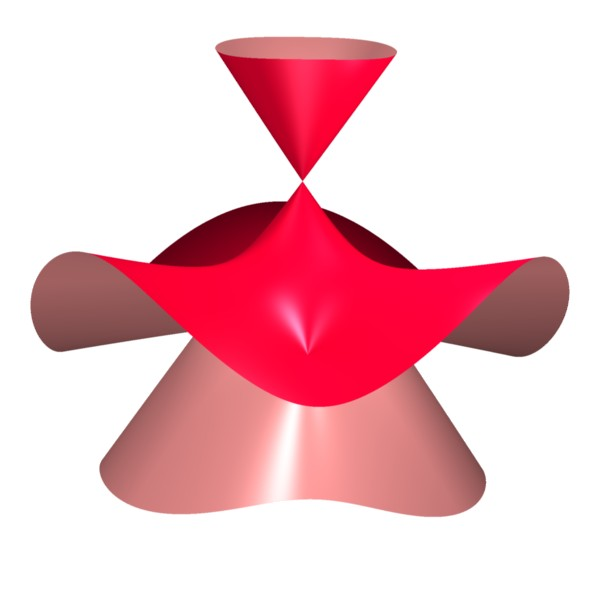
\includegraphics[width=1.35cm]{../../common/images/cayley_cubic_0}
        \end{tabular}
        &
        \begin{tabular}{@{}c@{}}
          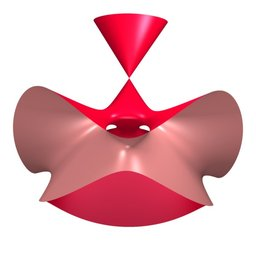
\includegraphics[width=1.35cm]{../../common/images/cayley_cubic_1}
        \end{tabular}
        &
        \begin{tabular}{@{}c@{}}
          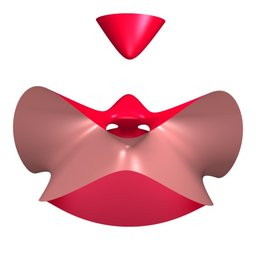
\includegraphics[width=1.35cm]{../../common/images/cayley_cubic_2}
        \end{tabular}
        &
        \begin{tabular}{@{}c@{}}
          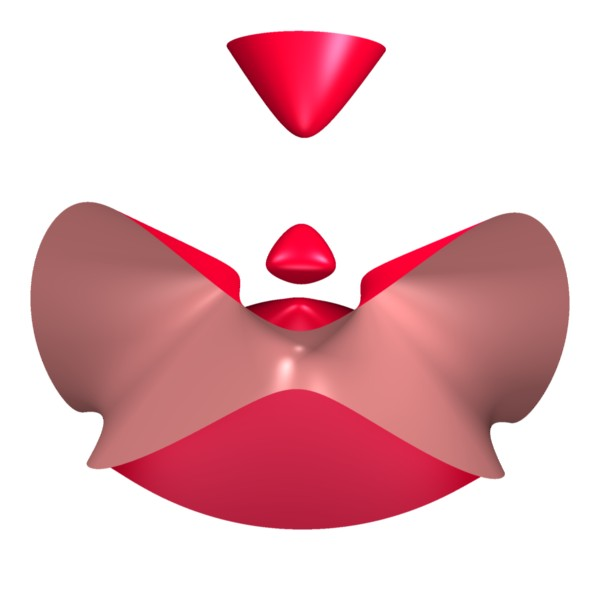
\includegraphics[width=1.35cm]{../../common/images/cayley_cubic_3}
        \end{tabular}
      \end{tabular}
    \end{center}
\end{surferPage}
